%!TEX program = xelatex

\documentclass[12pt,a4paper]{article}
\usepackage{xeCJK}
\usepackage{amsmath}
\setmainfont{Times New Roman}
\usepackage{setspace}
\usepackage{caption}
\usepackage{graphicx, subfig}
\usepackage{float}
\usepackage{listings}
\usepackage{booktabs}
\usepackage{setspace}%使用间距宏包
\usepackage{mathtools}
\usepackage{amsfonts}
\usepackage{amsmath}
    \newcommand{\dd}{\mathrm{d}}
\usepackage{tcolorbox}
    \tcbuselibrary{xparse}
        \DeclareTotalTCBox{\verbbox}{ O{green} v !O{} }
            {fontupper=\ttfamily,nobeforeafter,tcbox raise base,
             arc=0pt,outer arc=0pt,top=0pt,bottom=0pt,left=0mm,
             right=0mm,leftrule=0pt,rightrule=0pt,toprule=0.3mm,
             bottomrule=0.3mm,boxsep=0.5mm,bottomrule=0.3mm,boxsep=0.5mm,
             colback=#1!10!white,colframe=#1!50!black,#3}{#2}
\usepackage{color}
\usepackage{textcomp}
\definecolor{listinggray}{gray}{0.9}
\definecolor{lbcolor}{rgb}{0.9,0.9,0.9}
\lstset{
	backgroundcolor=\color{lbcolor},
	tabsize=4,
	rulecolor=,
	language=matlab,
        basicstyle=\scriptsize,
        upquote=true,
        aboveskip={1.5\baselineskip},
        columns=fixed,
        showstringspaces=false,
        extendedchars=true,
        breaklines=true,
        prebreak = \raisebox{0ex}[0ex][0ex]{\ensuremath{\hookleftarrow}},
        frame=single,
        showtabs=false,
        showspaces=false,
        showstringspaces=false,
        identifierstyle=\ttfamily,
        keywordstyle=\color[rgb]{0,0,1},
        commentstyle=\color[rgb]{0.133,0.545,0.133},
        stringstyle=\color[rgb]{0.627,0.126,0.941},
}
\begin{document} 
\title{homework11}
	\author{11611118 郭思源}  
\begin{spacing}{1.5}%%行间距变为double-space

\section{Question 1}

Solve the ODE system as follows
\[
    \frac{\dd x}{\dd t} = - x + y, \quad
    \frac{\dd y}{\dd t} = - x - y
\]




\begin{equation*}
	\begin{aligned}
		x &=  -\frac{\dd y}{\dd t}-y \\
		\frac{\dd x}{\dd t} &= -\frac{\dd y}{\dd^2 t} -\frac{\dd y}{\dd t} = \frac{\dd y}{\dd t}+2y \\\\
		\frac{\dd y}{\dd^2 t} &+ 2\frac{\dd y}{\dd t} + 2y = 0 \\
		r^2 &+ 2r + 2 = 0 \\
		r_1 &= - 1 +  i, \quad r_2 = - 1 -  i \\
		\alpha &= -1, \quad \beta = 1 \\
		y &= e^{\alpha t}(C_1\cos(\beta t)+C_2\sin(\beta t)) \\
		y &= e^{-t}(C_1\cos(t)+C_2\sin(t)) \\\\
	\end{aligned}
\end{equation*}

\begin{equation*}
	\begin{aligned}
		\frac{\dd y}{\dd t} &= e^{-t}(C_1(-\sin(t)-\cos(t))+C_2(\cos(t)-\sin(t)))\\
		x &=  -\frac{\dd y}{\dd t}-y =  e^{-t}(C_1\sin(t)-C_2\cos(t)) \\
	\end{aligned}
\end{equation*}

\begin{equation*}
	\begin{aligned}
		C_1 &= 1 \\
		C_2 &= 0 \\
		x(t) &= e^{-t}\sin(t) \\
		y(t) &= e^{-t}\cos(t) \\
	\end{aligned}
\end{equation*}


\section{Question 2}

Try the \verbbox{MATLAB} ODE solver by implementing the three numerical examples in the lecture note.

\subsection{Example model 1}
\[
    \frac{\dd x}{\dd t} = - x + y, \quad
    \frac{\dd y}{\dd t} = - x - y
\]
Let $x_0=0, y_0=1, t_0=0, t_e=1000$ :
\begin{lstlisting}[language=matlab]
function dydt = m1func(t,Y)
    x = Y(1);y = Y(2);
    dydt = [- x + y;
            - x - y];

[t xy]=ode45(@m1func,[0:0.01:1000],[0,1]);
x=xy(:,1);y=xy(:,2);
figure(1); plot(x,y);xlabel("x");ylabel("y");
\end{lstlisting}
\begin{figure}[htbp]
	\centering
	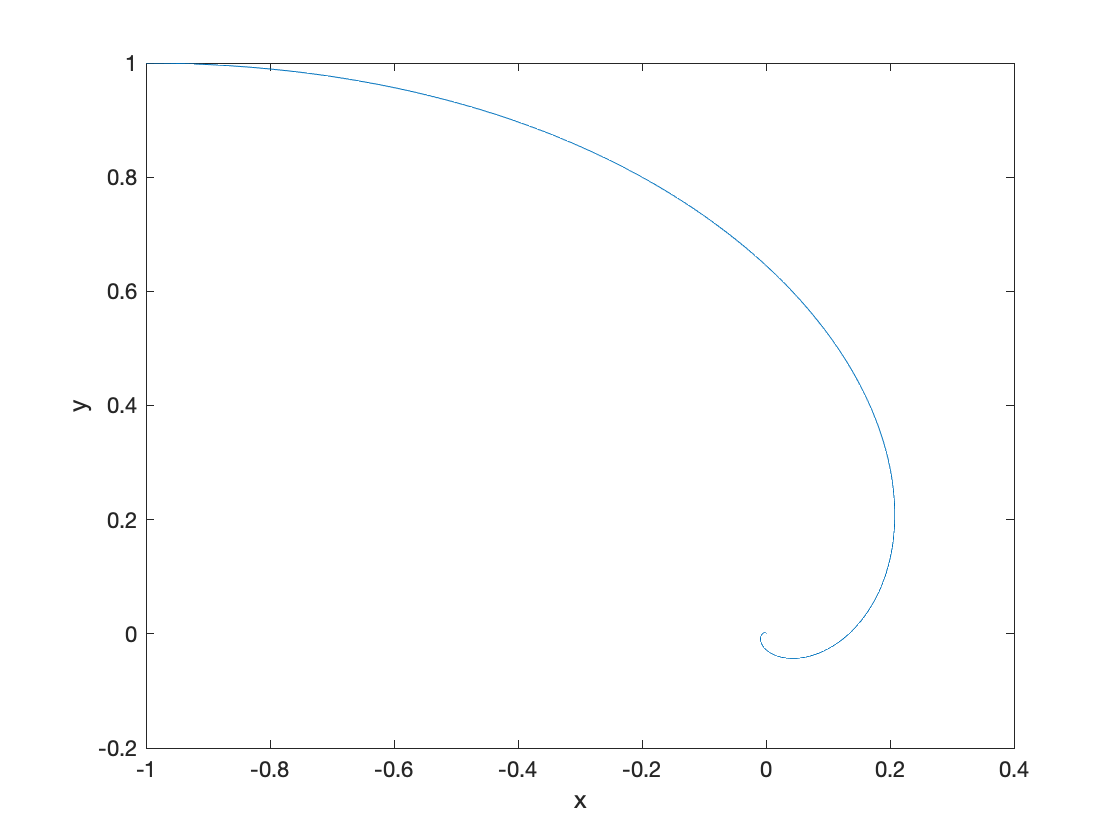
\includegraphics[scale=0.25]{m1.png}	
\end{figure}

\subsection{Example model 2}
\[
    \frac{\dd x}{\dd t} = ax - bxy, \quad
    \frac{\dd y}{\dd t} = my - nxy
\]
Let $a=1,b=100,m=1,n=100,\\ x_0=1, y_0=1, t_0=0, t_e=10000$ :

\begin{lstlisting}[language=matlab]
function dydt = m2func(t,Y)
    a = 1;b = 100;m = 1;n = 100;
    x = Y(1);y = Y(2);
    dydt = [a * x - b * x * y;
            m * y - n * x * y];

[t xy]=ode45(@m2func,[0:10000],[1,1]);

x=xy(:,1);y=xy(:,2);
figure(1); plot(x,y);xlabel("x");ylabel("y");
\end{lstlisting}
\begin{figure}[htbp]
	\centering
	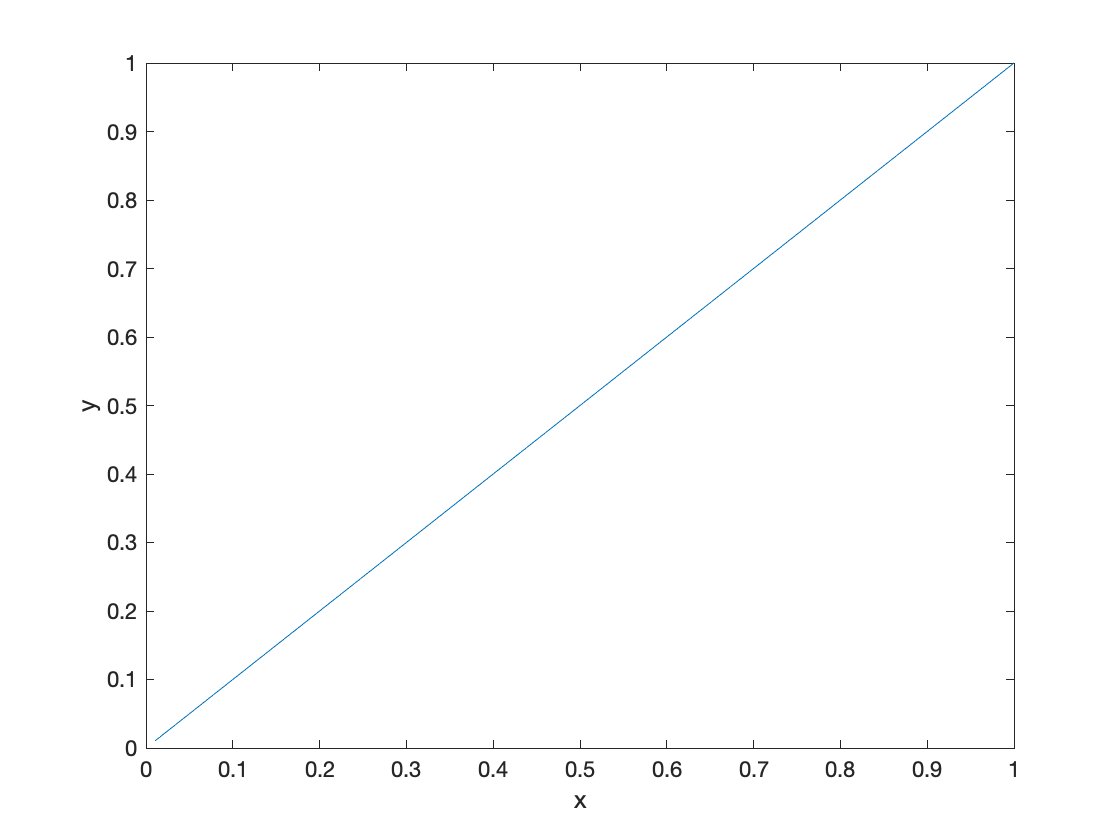
\includegraphics[scale=0.3]{m2.png}	
\end{figure}

\subsection{Example model 3}
\[
    \frac{\dd x}{\dd t} = - ax + by + c, \quad
    \frac{\dd y}{\dd t} = mx - ny + p
\]
Let $a=1,b=1,c=1,m=1,n=1,p=1 \\ x_0=1, y_0=1, t_0=0, t_e=10000$ :

\begin{lstlisting}[language=matlab]
function dydt = m3func(t,Y)
    a = 1;b = 1;c = 1;m = 1;n = 1;p = 1;
    x = Y(1);y = Y(2);
    dydt = [- a * x + b * y + c;
            m * x - n * y + p];

[t xy]=ode45(@m3func,[0:10000],[1,1]);

x=xy(:,1);y=xy(:,2);
figure(1); plot(x,y);xlabel("x");ylabel("y");
\end{lstlisting}
\begin{figure}[htbp]
	\centering
	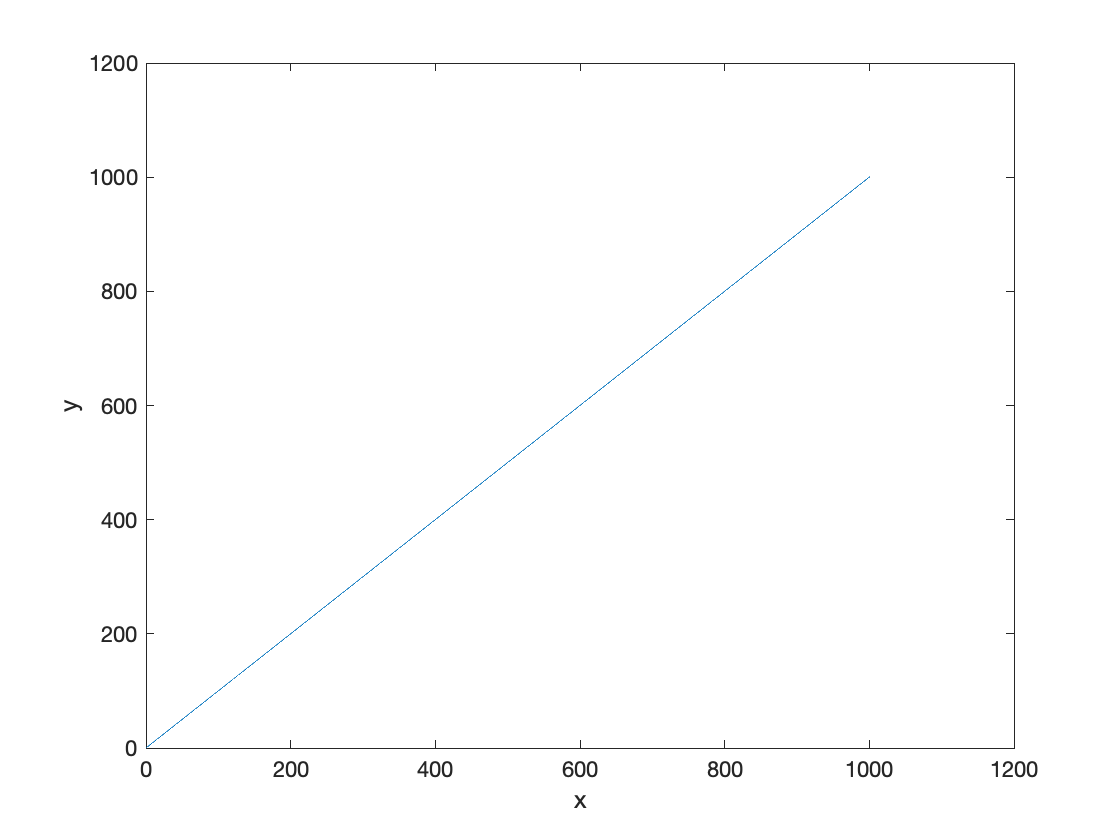
\includegraphics[scale=0.3]{m3.png}	
\end{figure}


\end{spacing}

\end{document}